\section{\dataset Benchmark}
% 加web说明
We introduce the \dataset benchmark, which contains 1200 real-world computer use tasks executed across Linux, Windows, macOS, Android, iOS, and cross-platform workflows.~\footnote{Due to copyright issues, Windows tasks require activation by the user, macOS and iOS tasks require Apple hardware.} Each task includes a natural-language goal, a reproducible initialization procedure, and a final-state evaluator.

\subsection{Operating System and Software Environments}

\dataset supports all mainstream operating systems, including \textbf{{desktop operating systems (Windows\windowsicon, macOS\macicon, Ubuntu\linuxicon)}}, \textbf{\textit{mobile operating systems (iOS\iosicon, Android\androidicon)}}, \textbf{{web (Chrome\chromeicon, Safari\safariicon)}}, and \textbf{{workflows that cross platforms}}. All platforms share the same specification format, while each platform retains the runtime mechanisms required by its own software stack. As shown in Figure~\ref{fig:distribution}, \dataset covers the most common categories of applications used in everyday digital life. Each example of these applications is shown in Appendix~\ref{app:more_task_examples}. 
% The desktop tasks including office editing, email, programming, graphics, diagrams, finance, media, reference management, maps, network analysis, shopping, and chat. Representative applications include LibreOffice, Thunderbird, GIMP, Blender, Wireshark, Zotero, Actual Budget, draw.io, VS Code, Notepad-like editors, Spotube, Delta Chat, and Marble. The mobile tasks including mail, messaging, notes, local storage, calendars, reminders, finance, browsing, shopping, galleries, music, and task management through applications such as K-9 Mail, Delta Chat, Markor, Fossify apps, Material Files, Oinkoin, Tasks.org, LibreOffice Viewer, Safari, FSNotes, Flow, Habit, and Maily.


% \begin{table*}[t]
\centering
\scriptsize
\setlength{\tabcolsep}{3.4pt}
\renewcommand{\arraystretch}{1.15}
\caption{Comparison with representative executable GUI-agent benchmarks. OS-OMNI covers desktop, mobile, web, and cross-platform workflows, enabling unified evaluation of generalist GUI agents across heterogeneous operating systems and applications.}
\label{tab:benchmark_comparison}
\resizebox{\textwidth}{!}{
\begin{tabular}{lccccccccccc}
\toprule
\multirow{2}{*}{\textbf{Benchmark}} &
\multirow{2}{*}{\makecell{\textbf{\# Tasks} \\}} &
\multicolumn{6}{c}{\textbf{Platform}} &
\multirow{2}{*}{\makecell{\textbf{Cross-} \\ \textbf{Platform}}} &
\multirow{2}{*}{\makecell{\textbf{Cross-} \\ \textbf{App}}} &
\multirow{2}{*}{\makecell{\textbf{Curated} \\ \textbf{Apps}}} &
\multirow{2}{*}{\makecell{\textbf{\# Apps} \\ \textbf{/ Sites}}} \\
\cmidrule(lr){3-8}
& &
\textbf{Win.} &
\textbf{Linux} &
\textbf{macOS} &
\textbf{iOS} &
\textbf{Android} &
\textbf{Web} &
& & & \\
\midrule

WorkArena~\citep{drouin2024workarena} &
33 &
\xmark & \xmark & \xmark & \xmark & \xmark & \cmark &
\xmark &
\xmark &
\xmark &
1 \\

WebArena~\citep{zhou2023webarena} &
812 &
\xmark & \xmark & \xmark & \xmark & \xmark & \cmark &
\xmark &
\xmark &
\xmark &
6 \\

VisualWebArena~\citep{koh2024visualwebarena} &
910 &
\xmark & \xmark & \xmark & \xmark & \xmark & \cmark &
\xmark &
\xmark &
\xmark &
3 \\

AndroidWorld~\citep{rawles2024androidworld} &
116 &
\xmark & \xmark & \xmark & \xmark & \cmark & \xmark &
\xmark &
\cmark &
\xmark &
20 \\

WindowsAgentArena~\citep{bonatti2024windows} &
154 &
\cmark & \xmark & \xmark & \xmark & \xmark & \cmark &
\xmark &
\cmark &
\xmark &
11 \\

AssistGUI~\citep{gao2023assistgui} &
100 &
\cmark & \xmark & \xmark & \xmark & \xmark & \xmark &
\xmark &
\xmark &
\xmark &
9 \\

WorldGUI~\citep{zhao2025worldgui} &
611 &
\cmark & \xmark & \xmark & \xmark & \xmark & \cmark &
\xmark &
\xmark &
\xmark &
10 \\

macOSWorld~\citep{yang2025macosworld} &
202 &
\xmark & \xmark & \cmark & \xmark & \xmark & \xmark &
\xmark &
\cmark &
\xmark &
30 \\

OSWorld~\citep{xie2024osworld} &
369 &
\cmark & \cmark & \cmark & \xmark & \xmark & \cmark &
\xmark &
\cmark &
\xmark &
9 \\

ScienceBoard~\citep{sun2025scienceboard} &
169 &
\xmark & \cmark & \xmark & \xmark & \xmark & \xmark &
\xmark &
\cmark &
\xmark &
6 \\

MMBench-GUI~\citep{wang2025mmbench} &
967 &
\cmark & \cmark & \cmark & \xmark & \cmark & \cmark &
\xmark &
\cmark &
\xmark &
-- \\

OS-MAP~\citep{chen2025map} &
416 &
\xmark & \cmark & \xmark & \xmark & \xmark & \cmark &
\xmark &
\cmark &
\xmark &
15 \\

\midrule
\textbf{OS-OMNI} &
\textbf{1200} &
\cmark & \cmark & \cmark & \cmark & \cmark & \cmark &
\cmark &
\cmark &
\cmark &
\textbf{35} \\
\bottomrule
\end{tabular}
}
% \vspace{0.3em}
\begin{flushleft}
\scriptsize
% \textbf{Note.} \cmark: supported; \xmark: not supported; \textbf{P}: partial support. ``Cross-Platform'' denotes workflows that span multiple operating systems or runtime environments, rather than merely evaluating separate tasks on different platforms. ``Curated Apps'' denotes benchmark-controlled applications or services with reproducible account/service state and final-state evaluation. Partial support indicates reliance on external real-account login or preloaded local account/profile state rather than benchmark-controlled account-service backends.
\end{flushleft}
\end{table*}


\begin{figure}[t]
    \centering
    \makebox[\textwidth][c]{%
        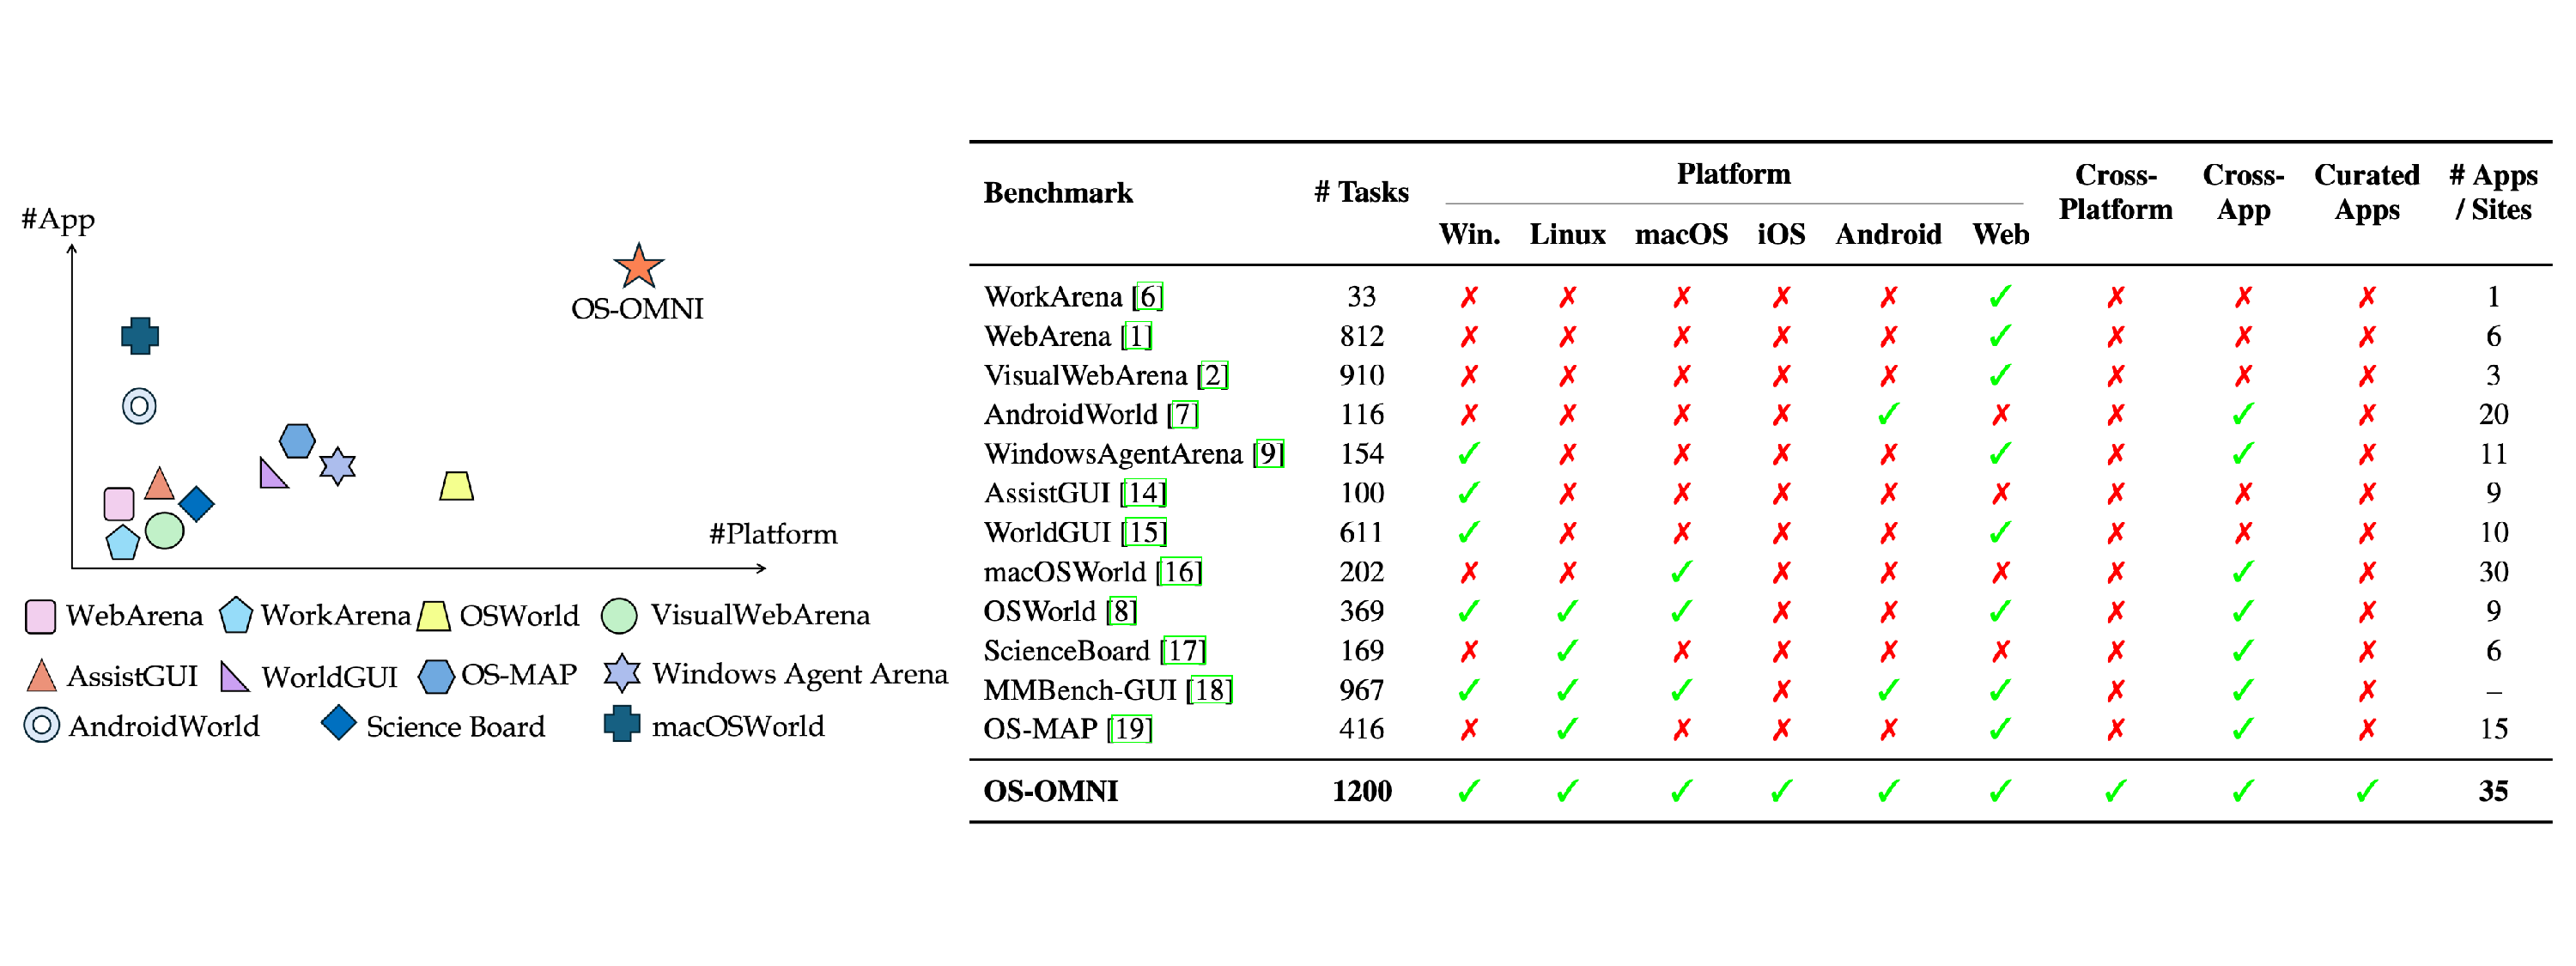
\includegraphics[width=1.2\textwidth]{figures/table1.pdf}
    }
    \caption{
Comparison with representative executable GUI-agent benchmarks. 
\#Platform indicates the number of supported platforms among Windows, Linux, macOS, iOS, Android, and Web, and \#App indicates the number of covered applications or websites. 
% For task properties, Cross-Platform denotes workflows spanning multiple operating systems or runtime environments, Cross-App denotes coordination across multiple applications, and Curated Apps denotes benchmark-controlled applications or services with reproducible account or service state and final-state evaluation. 
Compared with existing benchmarks, OS-OMNI provides broader platform coverage, richer application diversity, cross-platform workflows, and curated account-based service evaluation.
}
    \label{fig:comparison_benchmarks}
\end{figure}



\subsection{Custom Software for Controlled Application Coverage}
Real-world CUA workflows often involve applications that are difficult to include in benchmark environments. We address this issue by developing two types of custom software environments.

The first type targets service-oriented applications that are broadly important in everyday use but are usually excluded from existing benchmarks, such as online shopping, food ordering, or ride hailing. These scenarios require user accounts, payments, or unstable third-party backends, making them difficult to reproduce. To cover such workflows while preserving benchmark controllability, we built controlled applications that emulate login-based interactions. These applications provide realistic GUIs while keeping all data local or under the benchmark runtime, allowing reliable evaluation without depending on live commercial platforms or real user accounts.

The second type targets application domains that are available on some platforms with existing open-source software but are missing on others. Since \dataset aims to evaluate generalist CUA across desktop, mobile, and web platforms, we build additional platform-specific applications to fill these gaps and maintain comparable task coverage. This ensures that the benchmark evaluates generalist CUA capabilities under a shared task taxonomy, rather than being limited by the uneven availability of open-source applications on different operating systems.

\subsection{Tasks}
\vspace{-5pt}
\dataset consists of 1,200 meticulously curated CUA tasks across six platforms: \textbf{\textit{macOS}} (200), \textbf{\textit{Windows}} (200), \textbf{\textit{Ubuntu}} (200), \textbf{\textit{iOS}} (200), \textbf{\textit{Android}} (200), and \textbf{\textit{Web}} (200). The Web tasks are evenly distributed across the supported OS platforms and are instantiated through four widely used browsers: \textit{Chrome}, \textit{Edge}, \textit{Firefox}, and \textit{Safari}. Each task is represented by a specification that names the platform, instruction, initialization, and evaluator. Overall, the dataset construction was completed by 30 computer science graduate students over two months, with approximately 2,400 person-hours devoted to annotation and an additional 400 person-hours devoted to double-checking.

% \noindent
% \textbf{Task Annotation.}
% Our tasks are designed around software that annotators regularly use in their daily work, making them highly familiar with the corresponding interfaces, workflows, and practical usage patterns. In contrast, many existing benchmarks derive tasks from online tutorials, user guides, or documentation, which often leads to relatively basic and instructional scenarios. By leveraging real experience with these applications, our benchmark captures more realistic workflows and includes challenging tasks that better reflect how software is actually used in practice. The detailed examples of our task are shown in Appendix~\ref{}.  

% \noindent
% \textbf{Quality Control.} 
% To further control the quality of our data, we perform a five-stage data checking process. Each task is first constructed by an annotator with hands-on experience using the target software, ensuring that the workflow reflects realistic software usage. A second annotator then independently examines the task for clarity, feasibility, and potential ambiguity. Next, annotators calibrate task difficulty across platforms by comparing the expected number of human operation steps and revising accordingly. This calibration helps ensure that tasks from different platforms have approximately comparable human-step difficulty. We then use oracle trajectories to validate both the initializer and the evaluator. Specifically, the oracle execution is run from the initialized environment to verify that the task is solvable under the provided state, and the resulting final state is checked by the evaluator to ensure that a correct completion is reliably recognized. We further test representative failed or incomplete states to confirm that the evaluator rejects spurious solutions. Tasks whose initializer, instruction, difficulty level, or evaluator fails any of these checks are revised through additional inspection or removed from the benchmark.

\noindent
\textbf{Initial State Setup.}
Tasks rarely start from a blank desktop or a newly installed app. \dataset constructs these states in three stages: first restoring a platform baseline, then materializing task-specific data, and finally arranging the applications that the agent will observe. A task may restore a VM or simulator baseline, clone an execution template, reset selected applications, write files into the environment, seed application databases, configure local services, or place a transfer object for a subsequent phase. This design avoids storing a separate full-system image for every task while still allowing tasks to begin from realistic intermediate states.



\noindent
\textbf{Execution-based Evaluation.} 
\dataset uses final-state evaluators, which are executable scoring components selected by the task specification. The evaluations run guest-side checks, retrieve outputs from the runtime, parse application data, inspect local services, or compare generated objects against expected constraints. A successful task is therefore one whose final state satisfies the evaluator.

\subsection{Task Annotation Pipeline}
\label{sec:annotation_pipeline}

\begin{figure*}[t]
\centering
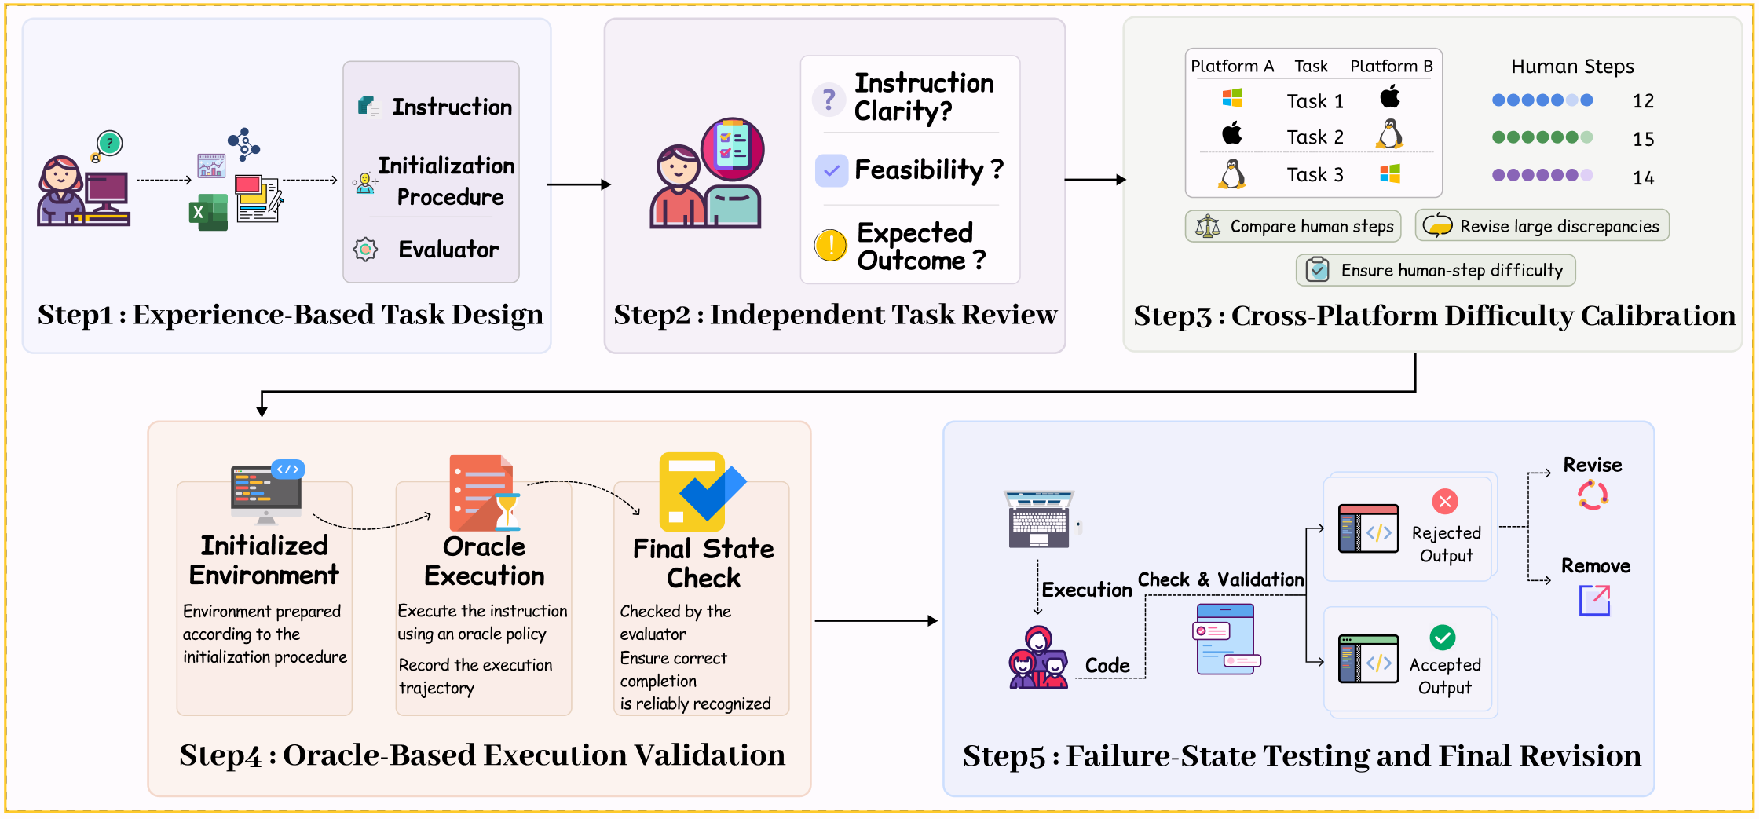
\includegraphics[width=\textwidth]{figures/annotation.pdf}
\caption{The five-stage task annotation pipeline for \dataset.}
\vspace{-15pt}
\label{fig:annotation}
\end{figure*}

As shown in Figure~\ref{fig:annotation}, we use a five-stages annotation pipeline:

(1) \textbf{Experience-Based Task Design.} Each task is constructed by an annotator with hands-on experience using the target software. The annotator designs a natural-language instruction together with the initialization procedure and evaluator. This stage ensures that the task is grounded in realistic software usage rather than being limited to basic operations.
(2) \textbf{Independent Task Review.} A second annotator examines each task for feasibility and ambiguity. This review checks whether the instruction is understandable, whether the task can be completed under the initialized environment, and whether the expected outcome is sufficiently well-defined for reliable evaluation.
(3) \textbf{Cross-Platform Difficulty Calibration.} Annotators then calibrate task difficulty across platforms by comparing the expected number of human operation steps required to complete each task. Tasks are revised when necessary to reduce large difficulty discrepancies, helping ensure that tasks from different platforms have comparable difficulty.
(4) \textbf{Oracle-Based Execution Validation.} We use oracle trajectories to validate both the initializer and the evaluator. Specifically, the oracle execution is run from the initialized environment to verify that the task is solvable under the provided state. The resulting final state is then checked by the evaluator to ensure that a correct completion is reliably recognized.
(5) \textbf{Failure-State Testing and Final Revision.} To further test evaluator robustness, we examine representative failed cases and verify that the evaluator rejects incorrect solutions. Tasks whose initializer, instruction, difficulty level, or evaluator fails any stage of the checking process are revised through additional inspection or removed from the benchmark.



\subsection{Data Statistics}

\begin{figure*}[t]
\centering
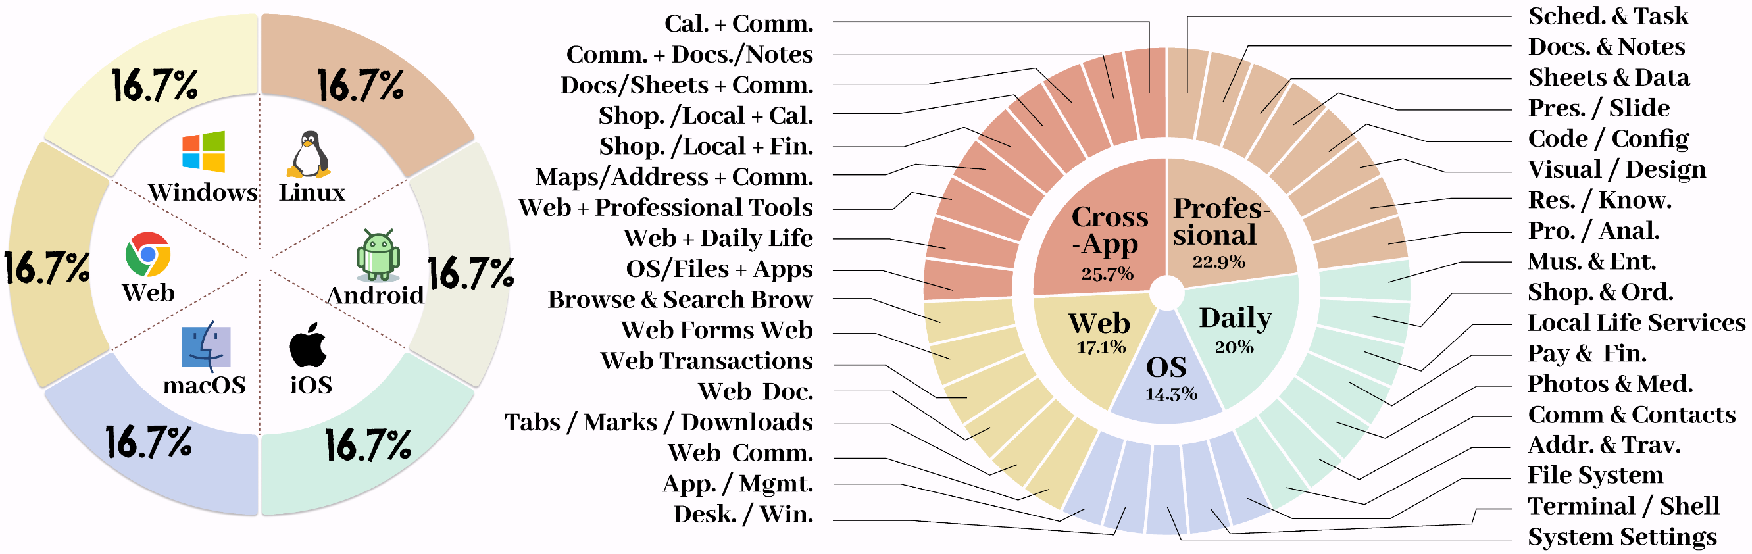
\includegraphics[width=\textwidth]{figures/stat.pdf}
\caption{\dataset contains 1,200 unique tasks in total, with 200 tasks for each platform: Windows, macOS, Ubuntu, iOS, Android, and Web.}
\vspace{-15pt}
\label{fig:distribution}
\end{figure*}
The main statistics of \dataset are summarized in Figure~\ref{fig:distribution}. \dataset contains 1,200 tasks, balanced across the five operating systems, web tasks are instantiated through browser environments on these platforms. The right chart in Figure~\ref{fig:distribution} summarizes the task taxonomy. At the coarse level, \dataset covers cross-application workflows (25.7\%), professional productivity tasks (22.9\%), daily-life tasks (20.0\%), web tasks (17.1\%), and operating-system tasks (14.3\%). We leave the complete fine-grained taxonomy and representative examples to Appendix~\ref{app:more_task_examples}.




\subsection{Comparison with existing benchmarks}
Figure~\ref{fig:comparison_benchmarks} compares \dataset with representative existing benchmarks in terms of platform coverage, task scale, application diversity, cross-platform workflows, cross-application workflows, and curated applications. WorkArena~\citep{drouin2024workarena}, WebArena~\citep{zhou2023webarena}, and VisualWebArena~\citep{koh2024visualwebarena} evaluate agents in web environments. AndroidWorld~\citep{rawles2024androidworld} focuses on Android. OSWorld~\citep{yang2025macosworld}, WindowsAgentArena~\citep{bonatti2024windows}, AssistGUI~\citep{gao2023assistgui}, WorldGUI~\citep{zhao2025worldgui}, macOSWorld~\citep{yang2025macosworld}, ScienceBoard~\citep{sun2025scienceboard}, MMBench-GUI~\citep{wang2025mmbench}, and OS-MAP~\citep{chen2025map} extend evaluation to desktop or multi-platform GUI settings, but they do not provide the same level of coverage across desktop, mobile, web, and cross-platform workflows.

In contrast, \dataset unifies Windows, Linux, macOS, iOS, Android, and Web environments under a single benchmark setting. It further introduces benchmark-controlled applications and services to support workflows involving persistent user state, backend records, shopping carts, orders, and payment-like options. Compared with benchmarks that rely on public websites, external accounts, or preloaded local profiles, this design enables reproducible initialization and reliable final-state evaluation without depending on live commercial platforms or real user accounts. As a result, \dataset evaluates agents on realistic service-oriented workflows that span multiple applications and platforms, rather than isolated GUI operations alone.